% =====================================================================
%  Section 8 (MERGED): Physics-Informed Conductivity from First Principles
%
%  Replaces the existing Section 8 ("Toward a Physics-Informed Conductivity
%  Model") AND the standalone "Ab Initio Deformation Potentials" draft.
%
%  Requires in preamble: amsmath, amssymb, graphicx, booktabs
%  (optional: siunitx, hyperref). If you do NOT use siunitx, replace every
%  \SI{x}{unit} with "x unit" and \si{...} accordingly.
%
%  Figures: drop your images at the Images/ paths marked below.
%  Citations: \cite{hamaguchi} = your current ref [3]; add yu_cardona,
%  herring_vogt, pollak_cardona for the literature comparison (bibtex provided
%  separately).
%
%  Search "% ADJUST" for choices to confirm:
%    - PBE equilibrium gap value (0.62 eV used)
%    - tense/voice (written as completed work)
%    - cross-reference labels to other sections
% =====================================================================


\section{Physics-Informed Conductivity from First Principles}
\label{sec:physics-informed}

The parametric study of Section~\ref{sec:parametric}% ADJUST: label of "Parametric Solution"
treated the coefficients $\pi$ and $\alpha$ in
\begin{equation}
  \sigma(\varepsilon) = \sigma_0\big(1 + \pi\,\varepsilon + \alpha\,\varepsilon^2 + \dots\big)
  \label{eq:sigma-taylor}
\end{equation}
as free phenomenological parameters. This section removes that freedom in two
steps. First, deformation-potential theory fixes the \emph{form} of
$\sigma(\varepsilon)$ and expresses $\pi,\alpha$ in terms of a single material
coupling, the hydrostatic deformation potential $(a_c+a_v)$. Second, that
coupling---together with the shear deformation potentials---is computed directly
from density-functional theory (DFT), so the constitutive law is fixed entirely
from first principles rather than fitted. The overall pipeline is
\begin{equation}
  \varepsilon \;\longrightarrow\; H_s \;\longrightarrow\; \Delta E_g(\varepsilon)
  \;\longrightarrow\; n(\varepsilon) \;\longrightarrow\; \sigma(\varepsilon)
  \;\longrightarrow\; \nabla\!\cdot\!\big(\sigma\nabla V\big)=0 ,
  \label{eq:pipeline}
\end{equation}
with each arrow developed below, following the treatment in Hamaguchi
\cite{hamaguchi}.
\subsection{Strain Hamiltonian and band-gap shift}
\label{subsec:strain-hamiltonian}

When a crystal is uniformly strained, the periodic potential seen by the
electrons changes, perturbing the Bloch Hamiltonian. To first order in strain
this perturbation is called the strain Hamiltonian $H_s$; it couples the
electronic degrees of freedom linearly to the strain tensor $\varepsilon_{ij}$
through the deformation-potential operator $D_{ij}$ \cite{hamaguchi}:
\begin{equation}
  H = H_0 + H_s, \qquad H_s = \sum_{i,j} D_{ij}\,\varepsilon_{ij}.
  \label{eq:Hs}
\end{equation}
Here $H_0$ is the unstrained Bloch Hamiltonian and $D_{ij}$ encodes how each
strain component modifies the crystal potential; its explicit form involves
derivatives of the ionic pseudopotential but need not be evaluated
directly---only its band-state matrix elements appear in what follows.
To first order, the shift of a non-degenerate band edge $|n\rangle$ follows
from perturbation theory,
\begin{equation}
  \Delta E_n = \langle n|H_s|n\rangle
             = \sum_{i,j}\langle n|D_{ij}|n\rangle\,\varepsilon_{ij}.
  \label{eq:dEn}
\end{equation}
Separating the strain into a hydrostatic part,
\begin{equation}
  \varepsilon_h = \varepsilon_{xx}+\varepsilon_{yy}+\varepsilon_{zz} = \operatorname{Tr}\varepsilon,
  \label{eq:eps-h}
\end{equation}
and traceless shear components, the hydrostatic part shifts the band edges
rigidly while the shear part lifts degeneracies. The shear-induced splitting,
parameterized by the deformation potentials $b$ (equivalently the uniaxial
potential $\Xi_u$) and $d$ in the Picus--Bir framework, is anisotropic and
underlies the dominant piezoresistive response of doped silicon; it is
quantified in Section~\ref{subsec:dft-results} and its route into transport is
discussed in Section~\ref{subsec:outlook}. The hydrostatic shift of the gap is
\begin{equation}
  \Delta E_g(\varepsilon_h) \approx (a_c+a_v)\,\varepsilon_h,
  \label{eq:gap-shift}
\end{equation}
where $a_c$ and $a_v$ are the hydrostatic deformation potentials of the
conduction and valence band edges \cite{hamaguchi}.

\subsection{From band shift to carrier density}
\label{subsec:carrier-density}

In the non-degenerate Maxwell--Boltzmann limit the conduction-band electron
concentration is
\begin{equation}
  n = N_c \exp\!\left(-\frac{E_c - E_F}{k_B T}\right),
  \label{eq:n-extrinsic}
\end{equation}
and for an intrinsic semiconductor charge neutrality fixes the Fermi level near
mid-gap, giving
\begin{equation}
  n_i = \sqrt{N_c N_v}\,\exp\!\left(-\frac{E_g}{2 k_B T}\right),
  \label{eq:n-intrinsic}
\end{equation}
so that the strain-induced gap shift~\eqref{eq:gap-shift} produces a
multiplicative change in $n_i$, with the factor $1/2$ inherited from the
square root.

\subsection{Strain-dependent conductivity}
\label{subsec:sigma-law}

Combining the Drude form $\sigma = n e^2 \tau / m^\ast$ with the intrinsic
carrier density~\eqref{eq:n-intrinsic} and the linear gap
shift~\eqref{eq:gap-shift}, and assuming the mobility prefactor $\tau/m^\ast$
varies weakly with strain,
\begin{equation}
  \sigma(\varepsilon) \approx
  \sigma_0 \exp\!\left(-\frac{\Delta E_g(\varepsilon)}{2 k_B T}\right)
  = \sigma_0 \exp\!\left(-\frac{(a_c+a_v)\,\varepsilon_h}{2 k_B T}\right),
  \label{eq:sigma-exp}
\end{equation}
where $\sigma_0$ absorbs the unstrained prefactors. Introducing the
dimensionless coupling
\begin{equation}
  \kappa \equiv \frac{a_c+a_v}{2 k_B T},
  \label{eq:kappa}
\end{equation}
expanding the exponential for $|\kappa\varepsilon_h|\ll 1$, and matching
term by term with~\eqref{eq:sigma-taylor} gives
\begin{equation}
  \pi = -\kappa = -\frac{a_c+a_v}{2 k_B T}, \qquad
  \alpha = \tfrac{1}{2}\kappa^2 = \tfrac{1}{2}\!\left(\frac{a_c+a_v}{2 k_B T}\right)^{\!2}.
  \label{eq:pi-alpha}
\end{equation}
Equation~\eqref{eq:pi-alpha} is the key link: the phenomenological coefficients
acquire a microscopic meaning, their sign and relative magnitude fixed by a
single material parameter. For typical semiconductors with $(a_c+a_v)>0$, the
linear coefficient $\pi$ is negative---tensile hydrostatic strain widens the gap
and lowers the intrinsic conductivity---and $\alpha = \tfrac12\pi^2$, so the two
coefficients are not independent.

\subsection{Sensitivity to the coupling strength}
\label{subsec:sensitivity}

Before fixing $(a_c+a_v)$ from DFT, it is useful to map how the response depends
on it. Table~\ref{tab:coupling-sweep} evaluates~\eqref{eq:pi-alpha} at
$T=\SI{300}{K}$ ($k_B T = \SI{0.0259}{eV}$) for three representative couplings.
Even a modest coupling of \SI{1}{eV} gives $|\pi|\approx19$, at the upper end of
the phenomenological range $\pi\in[5,20]$ used in Section~\ref{sec:parametric};
the first-principles value obtained below
(Section~\ref{subsec:firstprinciples-pi}) falls between the moderate and strong
cases.

\begin{table}[ht]
  \centering
  \begin{tabular}{lcccc}
    \toprule
    case & $a_c+a_v$ [eV] & $\varepsilon_0$ & $\pi$ & $\alpha$ \\
    \midrule
    weak     & 0.3 & $5\times10^{-3}$ & $-5.80$  & $1.68\times10^{1}$ \\
    moderate & 1.0 & $5\times10^{-3}$ & $-19.34$ & $1.87\times10^{2}$ \\
    strong   & 3.0 & $3\times10^{-3}$ & $-58.02$ & $1.68\times10^{3}$ \\
    \midrule
    \textbf{this work (DFT)} & \textbf{1.83} & $\le10^{-2}$ & $\mathbf{-35.4}$ & $\mathbf{6.3\times10^{2}}$ \\
    \bottomrule
  \end{tabular}
  \caption{Coefficients $\pi$ and $\alpha$ from~\eqref{eq:pi-alpha} at
  $T=\SI{300}{K}$. The first three rows are a sensitivity sweep over
  representative couplings; the last row uses the first-principles value
  $a_c+a_v=\SI{1.83}{eV}$ determined in Section~\ref{subsec:dft-results}.}
  \label{tab:coupling-sweep}
\end{table}

The exponential law~\eqref{eq:sigma-exp} and its Taylor
truncation~\eqref{eq:sigma-taylor} are compared in
Figure~\ref{fig:sigma-exp-taylor}. For weak and moderate coupling the two are
indistinguishable across $|\varepsilon|\le0.02$; for strong coupling the Taylor
form begins to miss the tensile/compressive asymmetry of the exponential.

\begin{figure}[ht]
  \centering
  %\includegraphics[width=0.8\linewidth]{Images/sigma_exp_taylor.png}
  \caption{Normalized conductivity $\sigma(\varepsilon)/\sigma_0$ versus strain
  for three couplings at $T=\SI{300}{K}$. Solid: exponential
  law~\eqref{eq:sigma-exp}; dashed: Taylor approximation~\eqref{eq:sigma-taylor}
  with the coefficients~\eqref{eq:pi-alpha}.}
  \label{fig:sigma-exp-taylor}
\end{figure}

\subsection{Coupled finite-element solution}
\label{subsec:coupled-fem}

The one-dimensional conductivity equation~\eqref{eq:1d-cond}% ADJUST: label of div(sigma grad V)=0
is solved with the physics-informed law~\eqref{eq:sigma-exp} for a prescribed
strain profile $\varepsilon(x)=\varepsilon_0\sin(\pi x)$ on $[0,1]$ with
$V(0)=0,\,V(1)=1$. The mechanical assembly, linear solve, and post-processing
are unchanged from Section~\ref{sec:parametric}; only the local material law is
replaced.

Figure~\ref{fig:fem-coupled} shows the moderate case
($a_c+a_v=\SI{1}{eV}$, $\varepsilon_0=5\times10^{-3}$): the strain modulates the
conductivity, the potential bows away from the linear baseline, the electric
field develops a compensating spatial variation, and the current density remains
constant to machine precision---the discrete statement of $\nabla\!\cdot\!J=0$
and the principal consistency check. The exponential and Taylor laws are
numerically indistinguishable at this amplitude, consistent
with~\eqref{eq:pi-alpha}. Figure~\ref{fig:fem-sweep} shows that the departure of
$V(x)$ and $E(x)$ from the uncoupled baseline grows with $(a_c+a_v)$.

\begin{figure}[ht]
  \centering
  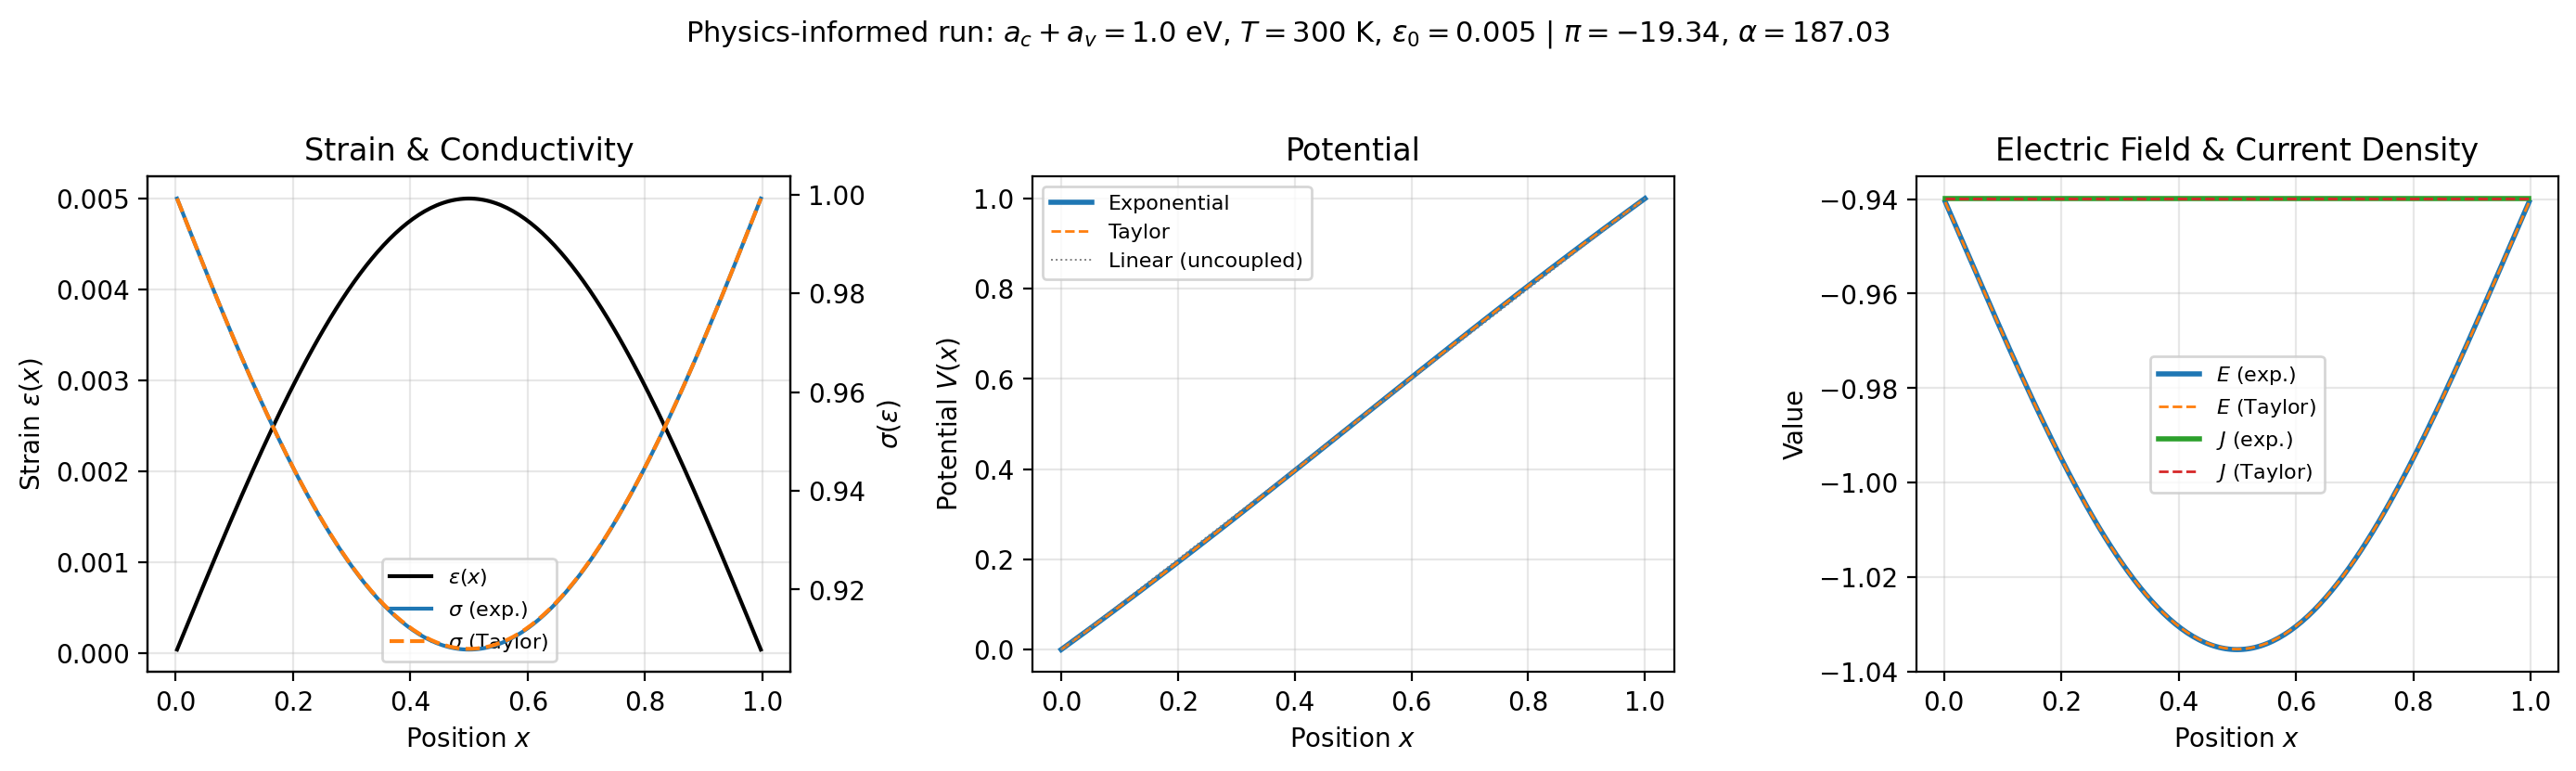
\includegraphics[width=0.95\linewidth]{Images/fig_FEM_moderate.png}
  \caption{Finite-element solution of the coupled problem with the
  physics-informed law~\eqref{eq:sigma-exp} for $a_c+a_v=\SI{1}{eV}$ at
  $T=\SI{300}{K}$, $\varepsilon_0=5\times10^{-3}$. Left: strain and conductivity;
  middle: potential; right: electric field and current density. $J$ is constant
  to machine precision while $E$ varies to compensate $\sigma(x)$.}
  \label{fig:fem-coupled}
\end{figure}

\begin{figure}[ht]
  \centering
  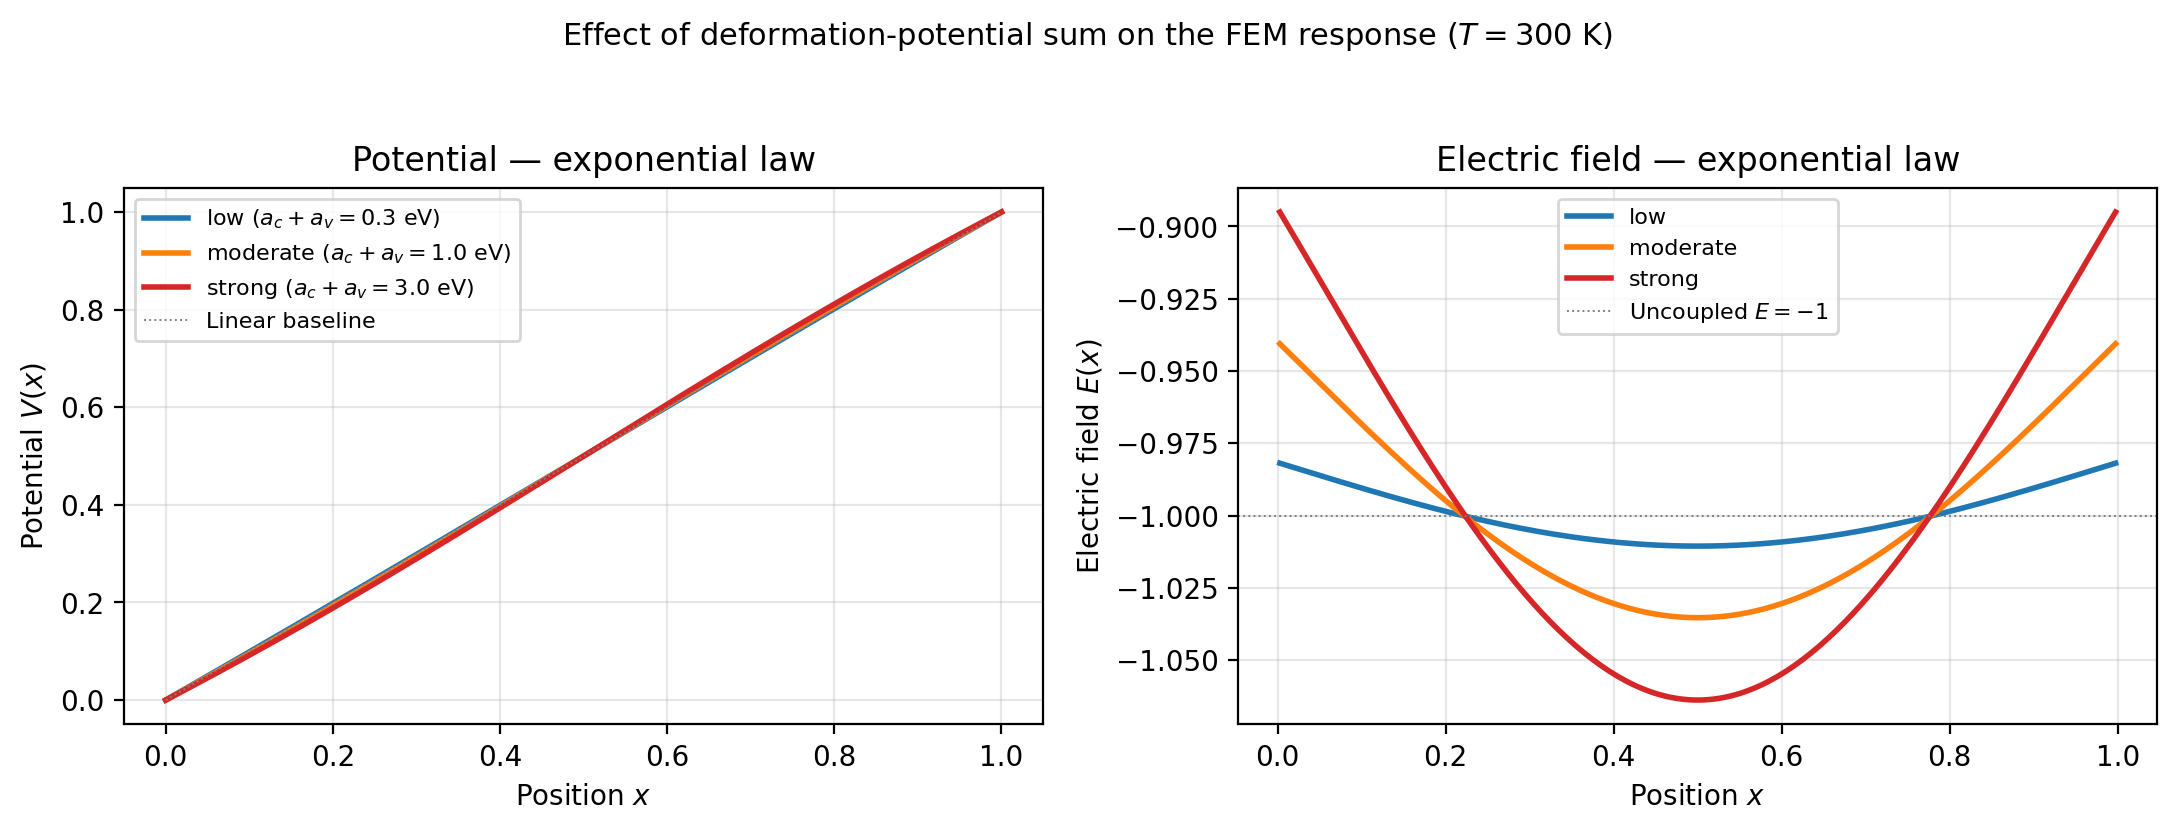
\includegraphics[width=0.95\linewidth]{Images/fig_compare_cases.png}
  \caption{Effect of the deformation-potential sum on the FEM response at
  $T=\SI{300}{K}$. Left: potential profiles for the three cases of
  Table~\ref{tab:coupling-sweep}; right: electric field. The deviation from the
  uncoupled value $E=-1$ grows with the coupling strength.}
  \label{fig:fem-sweep}
\end{figure}

% =====================================================================
%  DETERMINATION HALF — first-principles DFT
% =====================================================================

\subsection{First-principles deformation potentials}
\label{subsec:dft-results}
The coupling $(a_c+a_v)$ used above is only one of three independent deformation
potentials of cubic silicon. The other two---the uniaxial potential $\Xi_u$ and
the shear potential $d$---do not enter the scalar law~\eqref{eq:sigma-exp}, but
they govern the dominant, anisotropic part of silicon's piezoresistance through
valley repopulation and valence-band splitting (Section~\ref{subsec:outlook}).
All three are computed here from the band structure: the hydrostatic potential to
fix the constitutive law, and the shear potentials to supply the inputs the full
transport treatment requires. The physical chain is exactly the
pipeline~\eqref{eq:pipeline}: applied strain moves the atoms, which changes the
potential the electrons feel, which shifts and splits the bands; the slopes of
those shifts with respect to strain are the deformation potentials. Cubic symmetry
fixes how many are independent and which strain isolates each one.

\paragraph{One strain mode per deformation potential.}
A general strain of silicon separates into three symmetry-distinct modes, each
isolating one deformation potential (Table~\ref{tab:strain-modes}). This is what
makes the calculation efficient: three symmetry-pure strains suffice, rather
than a scan over arbitrary deformations.

\begin{table}[ht]
  \centering
  \begin{tabular}{lll}
    \toprule
    Strain mode & Effect on the bands & Probes \\
    \midrule
    Hydrostatic (volume) & gap shifts, no splitting          & $a = a_c+a_v$ \\
    Tetragonal (one axis) & $\langle100\rangle$ valleys split & $\Xi_u$ \\
    Trigonal shear (angles) & valence top at $\Gamma$ splits  & $d$ \\
    \bottomrule
  \end{tabular}
  \caption{The three symmetry-pure strain modes and the deformation potential
  each isolates. Hydrostatic strain keeps all directions equivalent (no
  splitting); the tetragonal and shear modes break symmetry and lift specific
  degeneracies.}
  \label{tab:strain-modes}
\end{table}

\paragraph{Computational method.}
Calculations use VASP with PAW PBE potentials, a plane-wave cutoff of
\SI{320}{eV}, and the relaxed primitive cell of silicon as the
$\varepsilon=0$ reference. Crystal symmetry is disabled (\texttt{ISYM}=0) so that
a small symmetry-lowering strain is not folded back to the cubic structure,
which would erase the splitting being measured. Each strained structure is run
in stages: a self-consistent calculation on a uniform $\mathbf k$-mesh converges
the charge density, then a non-self-consistent calculation produces the bands
along a high-symmetry path. For the trigonal-shear runs an ionic relaxation at
fixed cell shape precedes these steps, because the two atoms of the diamond
basis displace relative to one another under shear (the internal-strain or
Kleinman effect); the hydrostatic and tetragonal modes need no such relaxation.
Strain amplitudes of $\pm0.2,0.5,1.0\,\%$ are applied, and each deformation
potential is obtained as the slope of a band feature versus strain. The
equilibrium PBE band structure is shown in Figure~\ref{fig:bands-eq}; PBE
underestimates the absolute gap ($E_g(0)\approx\SI{0.62}{eV}$% ADJUST: PBE gap value
versus the experimental \SI{1.12}{eV}), but the deformation potentials are
\emph{slopes} and are far less sensitive to this error than the absolute gap. 
\begin{RL}
However one can use corrections for example in \cite{DFT_Correction}.
\end{RL}

\begin{figure}[ht]
  \centering
  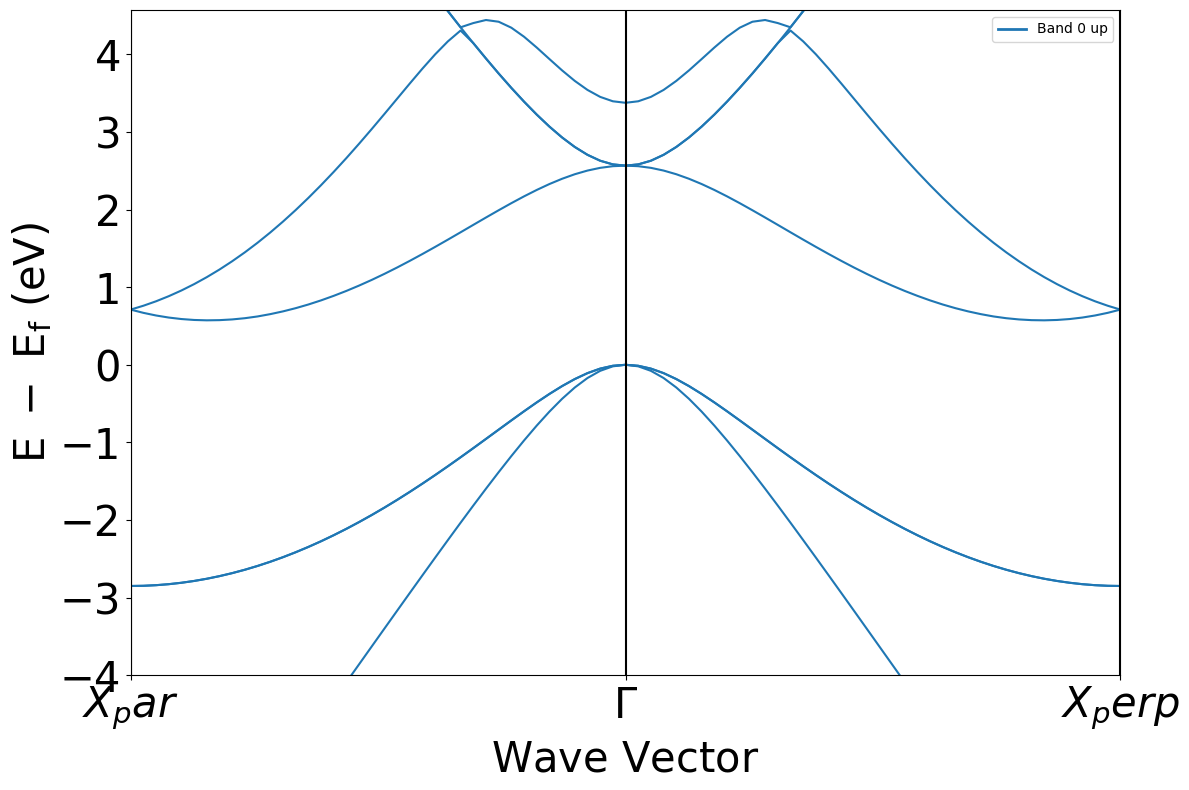
\includegraphics[width=0.75\linewidth]{Images/bands_equilibrium.png}
  \caption{Equilibrium band structure of silicon (VASP, PBE) along the
  dual-X path $X_\parallel$--$\Gamma$--$X_\perp$, energies referenced to the
  valence-band maximum. At zero strain the two X points are degenerate; the
  valence maximum sits at $\Gamma$ and the conduction minima near $X$,
  reproducing the indirect gap.}
  \label{fig:bands-eq}
\end{figure}

\paragraph{Extraction and results.}
The extraction relations follow from the band features in
Table~\ref{tab:strain-modes}:
\begin{align}
  a = a_c+a_v &= \frac{\mathrm{d}E_g}{\mathrm{d}\,\operatorname{Tr}\varepsilon}, \\[2pt]
  \Xi_u &= \frac{\mathrm{d}}{\mathrm{d}\varepsilon}\big[E_c(X_\parallel)-E_c(X_\perp)\big], \\[2pt]
  |d| &= \frac{\Delta E_{\Gamma_{25'}}}{3\sqrt{3}\,\varepsilon_{xy}} .
\end{align}
The band structures for the three modes at $\varepsilon=-1\%,0,+1\%$ are shown
in Figure~\ref{fig:bands-modes}, and the linear fits behind each potential in
Figure~\ref{fig:dp-extraction}. The resulting values are collected in
Table~\ref{tab:dp-values}.

\begin{figure}[ht]
  \centering
  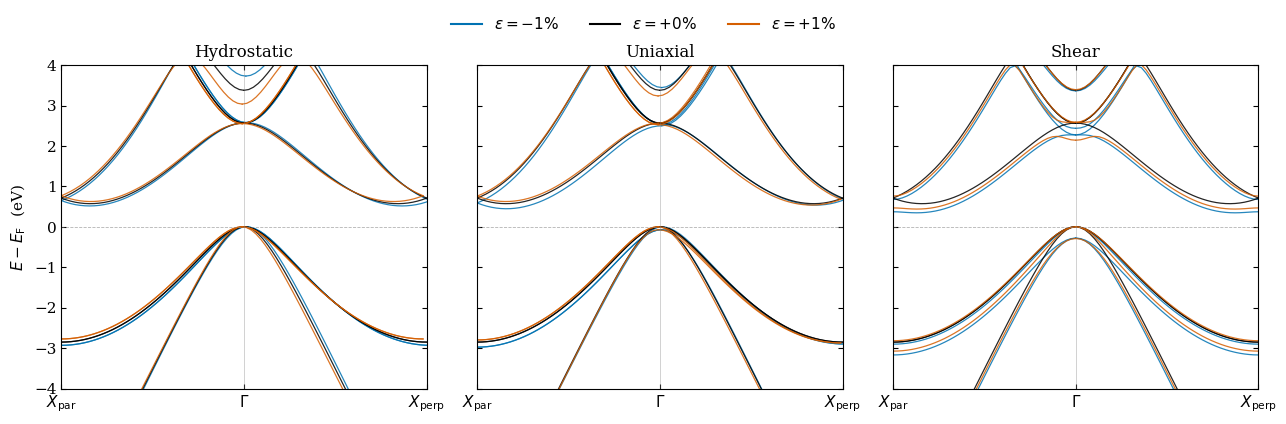
\includegraphics[width=0.95\linewidth]{Images/bands_strain_modes.png}
  \caption{Band structure of silicon at $\varepsilon=-1\%,0,+1\%$ for the three
  strain modes. Hydrostatic strain shifts the gap with no splitting; tetragonal
  strain splits the conduction valleys ($X_\parallel$ vs.\ $X_\perp$); trigonal
  shear splits the valence-band maximum at $\Gamma$.}
  \label{fig:bands-modes}
\end{figure}

\begin{figure}[ht]
  \centering
  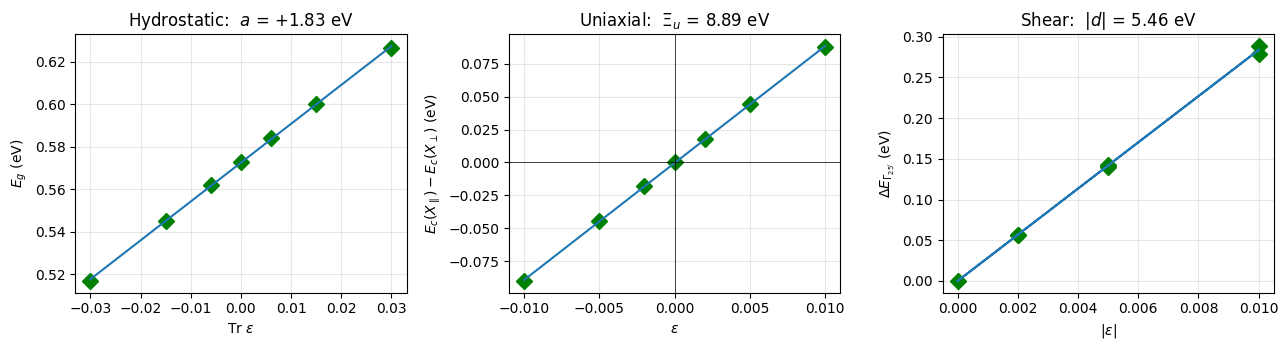
\includegraphics[width=0.95\linewidth]{Images/dp_extraction.png}
  \caption{Deformation potentials as slopes: gap versus hydrostatic strain
  ($a$); valley splitting versus tetragonal strain ($\Xi_u$), passing through
  zero at $\varepsilon=0$; valence splitting versus shear magnitude ($|d|$). The
  slopes give the values of Table~\ref{tab:dp-values}.}
  \label{fig:dp-extraction}
\end{figure}

\begin{table}[ht]
  \centering
  \begin{tabular}{llll}
    \toprule
    Deformation potential & This work & Literature (Si) & Source \\
    \midrule
    $a = a_c+a_v$            & $+1.83$ eV       & $\sim +1.5$       & \cite{yu_cardona} \\
    $\Xi_u$                  & $+8.89$ eV       & $9.0 \pm 2$       & \cite{yu_cardona, herring_vogt} \\
    $|d|$                    & $5.46$ eV        & $\sim 5.3\;(d<0)$ & \cite{yu_cardona, pollak_cardona} \\
    $\mathrm{d}E_g/\mathrm{d}P=-a/B$ & $-18.7$ meV/GPa & $\sim -15$ & \cite{yu_cardona} \\
    \bottomrule
  \end{tabular}
  \caption{Deformation potentials of silicon from the three strain sweeps,
  compared with literature. The gap potential $a$ carries its sign because it
  sets the sign of $\pi$ via~\eqref{eq:pi-alpha}; $\Xi_u$ is a positive splitting
  coefficient; $d$ is reported as a magnitude, the standard convention being
  $d<0$. The pressure coefficient $\mathrm{d}E_g/\mathrm{d}P=-a/B$ (bulk modulus
  $B\approx\SI{98}{GPa}$) is a convention-independent comparison with experiment.}
  \label{tab:dp-values}
\end{table}

Each sweep reproduces the behaviour symmetry requires, which validates the
calculation independently of the fitted numbers. Hydrostatic strain shifts the
gap monotonically with no splitting; tetragonal strain produces a valley
splitting that vanishes at $\varepsilon=0$ and reverses sign with the strain (the 
transverse valleys forming the conduction minimum under tension, the strain-axis valleys under compression); trigonal
shear splits the $\Gamma_{25'}$ valence triplet symmetrically in $\pm\varepsilon$,
the signature of a pure traceless shear. The negative pressure coefficient,
close to the measured value, confirms the full chain from atomic structure to
band gap.
\subsection{First-principles \texorpdfstring{$\pi$}{pi}
            and \texorpdfstring{$\alpha$}{alpha}}
\label{subsec:firstprinciples-pi}

Inserting the computed $a=a_c+a_v=\SI{1.83}{eV}$ into~\eqref{eq:kappa}
and~\eqref{eq:pi-alpha} at $T=\SI{300}{K}$ gives
\begin{equation}
  \kappa = \frac{a_c+a_v}{2k_BT} = 35.4, \qquad
  \pi = -35.4, \qquad
  \alpha = \tfrac12\kappa^2 = 626.
  \label{eq:firstprinciples-pi}
\end{equation}
This is the last row of Table~\ref{tab:coupling-sweep}: silicon sits between the
moderate and strong cases, the coupling is sizeable, and the negative sign
confirms that tensile hydrostatic strain lowers the intrinsic conductivity. The
representative parameters of Section~\ref{sec:parametric} are thereby replaced by
a single computed value, and the hydrostatic part of $\sigma(\varepsilon)$
in~\eqref{eq:sigma-exp} is fixed entirely from first principles.
Figure~\ref{fig:fem-coupled2} shows the resulting finite-element solution;
the potential deviates visibly from the uncoupled baseline, confirming that
$a=\SI{1.83}{eV}$ produces a physically meaningful piezoresistive response.

\begin{figure}[ht]
  \centering
  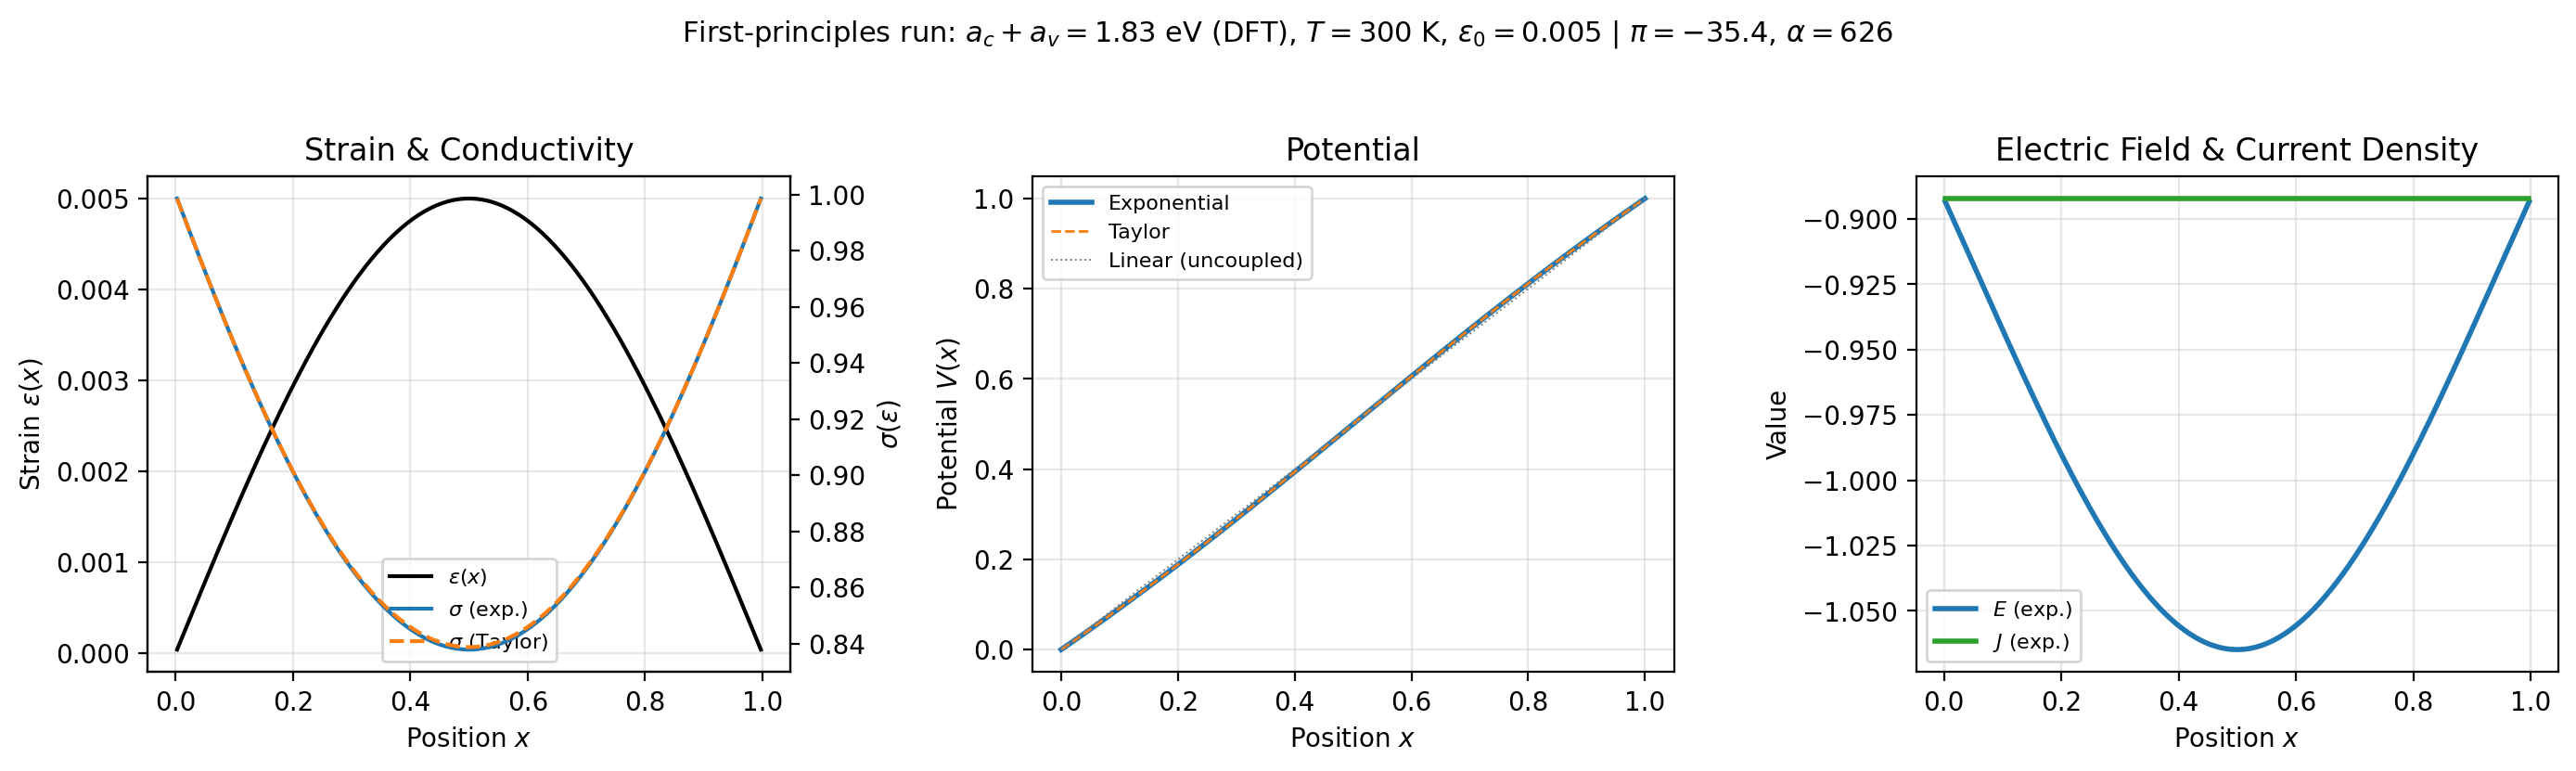
\includegraphics[width=0.95\linewidth]{Images/fem_dft.png}
  \caption{Finite-element solution with the physics-informed
  law~\eqref{eq:sigma-exp} for $a_c+a_v=\SI{1.83}{eV}$ (DFT, $\pi=-35.4$,
  $\alpha=626$) at $T=\SI{300}{K}$, $\varepsilon_0=5\times10^{-3}$. Left: strain
  and conductivity; middle: potential; right: electric field and current density.
  $J$ is constant to machine precision while $E$ compensates $\sigma(x)$,
  completing the first-principles pipeline~\eqref{eq:pipeline}.}
  \label{fig:fem-coupled2}
\end{figure}
\subsection{Outlook: the transport step and the role of shear strain}
\label{subsec:outlook}

The constitutive law developed above is complete and self-contained, but it
captures only one of the two channels through which strain alters conductivity,
and not the dominant one for the devices of interest.

\paragraph{Two channels, one implemented.}
Through $\sigma = n e \mu$, strain can act on the carrier density $n$ or on the
mobility $\mu$. The exponential law~\eqref{eq:sigma-exp} is the \emph{density}
channel: hydrostatic strain shifts the gap, the gap shifts $n$ through
Maxwell--Boltzmann statistics, and only the hydrostatic potential $a=a_c+a_v$
enters. This channel is isotropic by construction---it depends on $\varepsilon$
only through the scalar $\operatorname{Tr}\varepsilon$---and is sub-dominant in
doped silicon, where $n\approx N_D$ is pinned by the dopants and responds only
weakly to a gap shift.

\paragraph{Why the shear potentials were computed.}
The large, technologically exploited piezoresistance of silicon, first measured
by Smith \cite{smith1954}, comes from the \emph{mobility} channel and is anisotropic.
Uniaxial $\langle100\rangle$ strain splits the six conduction valleys (coefficient
$\Xi_u$); electrons repopulate toward the lowered valleys, changing the
direction-averaged conductivity mass and hence $\mu$. This is the origin of the
large $\pi_{11}$ of $n$-type silicon. Trigonal shear splits the valence-band
maximum (coefficient $d$), redistributing holes among bands of different
curvature, which dominates $\pi_{44}$ of $p$-type silicon. The potentials $\Xi_u$
and $d$ in Table~\ref{tab:dp-values} are therefore not auxiliary: they
parameterize the principal piezoresistive effect. They are absent from
$\sigma(\varepsilon)$ here only because the carrier-density argument has no place
for them---valley repopulation changes mobility, not carrier number.

\paragraph{Where the Boltzmann transport equation enters.}
Routing $\Xi_u$ and $d$ into transport requires the conductivity in its full
Boltzmann tensor form,
\begin{equation}
  \sigma_{ij} = \frac{e^2}{4\pi^3}\sum_n \int
  v^n_i(\mathbf k)\,v^n_j(\mathbf k)\,\tau_n(\mathbf k)
  \left(-\frac{\partial f_0}{\partial E}\right)\mathrm d\mathbf k ,
  \label{eq:bte-outlook}
\end{equation}
rather than the scalar $\sigma = ne\mu$. Strain enters~\eqref{eq:bte-outlook}
through the shifted band energies $\delta E_n = \Xi_{ij}\varepsilon_{ij}$, which
modify the group velocities $v^n_i=\hbar^{-1}\partial E_n/\partial k_i$, the
valley occupations through $-\partial f_0/\partial E$, and the intervalley
relaxation times $\tau_n$. The result is a genuine tensor
$\sigma_{ij}(\varepsilon)$ carrying the anisotropy that the scalar law cannot
represent. Equation~\eqref{eq:bte-outlook} requires two ingredients the present
work does not yet supply: the strained band structure on a dense $\mathbf k$-mesh,
available in principle from the same VASP runs used here, and the relaxation times
$\tau_n(\mathbf k)$, which demand a separate electron--phonon calculation
(density-functional perturbation theory coupled to a Boltzmann-transport solver).
The deformation potentials of Section~\ref{subsec:dft-results} are exactly the
band-structure inputs this step consumes; the relaxation times are the remaining
piece.

\paragraph{Further approximations.}
Two narrower assumptions accompany the density channel. The intrinsic carrier
density~\eqref{eq:n-intrinsic} overstates the gap contribution in doped devices,
where the mobility channel above dominates; and the Maxwell--Boltzmann
form~\eqref{eq:n-extrinsic} fails at high doping or low temperature, where
Fermi--Dirac statistics are required. Neither alters the structure of the
pipeline~\eqref{eq:pipeline} or the finite-element infrastructure of
Section~\ref{sec:parametric}: each refinement replaces the local material law
while leaving the assembly and solver untouched.



% =====================================================================
%  Uniaxial channel
% =====================================================================


\subsection{Uniaxial Channel: Valley Repopulation}
\label{subsec:uniaxial}

In hydrostatic channel we have developed through \ref{eq:Hs} (the trace part of 
strain tensor), the shift of bands calculations. We have also identified the anisotropic splitting
of the bands in traceless part of the tnesor. 

The route to transport for this part includes the electron mobility repopulation since the anisotropic
distribution of the valleys. This leads to study the redistribution of energy valleys, as an effect of 
applied uniaxial strain.


% [opening: contrast with hydrostatic — see rewrite below]

\paragraph{Symmetry of the six-valley splitting.} The uniaxial strain breaks the rotational symmetry(...). 
This leads to an anisotropic repopulation of the momenta along $<100>$, for Si and along $<111>$ for Ge /cite{hamaguchi}. 
%[the Herrin-Vogt term, the (100) grouping into 2+4, Table cross-ref]

\paragraph{Repopulation and the conductivity tensor.}
%[Boltzmann weights, cancellation of $a$, sigma = sum over six fixed M_i^{-1},
%the epsilon=0 isotropy gate as validation]

\paragraph{Extraction of $\pi_{11}-\pi_{12}$.}
%[strain-to-stress bridge, combined with the hydrostatic result to solve
%the 2x2 system, benchmark against Smith (1954)]

\paragraph{Role of the effective masses.}
%[m_l, m_t from DFT curvature at the valley minimum; note the classic
%cyclotron-resonance values this benchmarks against, \cite{hamaguchi} Eq. 2.26 —
%this is where your existing cyclotron-resonance sentence actually belongs,
%reframed as a validation check rather than a floating fact]